\documentclass[class=article, crop=false]{standalone}
\usepackage[subpreambles=true]{standalone}
\usepackage[a4paper]{geometry}
\usepackage{import}
\usepackage{ebproof}
\usepackage[utf8]{inputenc}
\usepackage{tikz}
\usepackage{hyperref}
\usepackage{amsmath}
\usepackage{amssymb}
\usepackage{listings}
\usepackage{verbatim}
\usepackage[super]{nth}
\usepackage{float}
\usepackage{subcaption}

\ifstandalone
\usepackage{color}
\usepackage{xcolor}
\usepackage{caption}
\usepackage{courier}

\lstdefinelanguage{efflang}
{
    % list of keywords
    morekeywords={
        let,
        perform,
        continue,
        val,
        effect,
        in,
        if, then, else,
        with, handle, handler,
        finally,
        match,
        exception,
        of
    },
    sensitive=false,
    morecomment=[s]{(*}{*)},
    morestring=[b]"
}

\lstdefinelanguage{scheme}
{
    % list of keywords
    morekeywords={
        define, call/cc, lambda
    },
    sensitive=false,
    morecomment=[s]{\#|}{|\#},
    morestring=[b]"
}

\lstset{
  basicstyle=\small\ttfamily, % Default font
  numberstyle=\small,          % Style of line numbers
  numbersep=5pt,              % Margin between line numbers and text
  tabsize=2,                  % Size of tabs
  extendedchars=true,
  breaklines=true,            % Lines will be wrapped
  keywordstyle=\color{red},
  frame=b,
  numbers=left,
  numberstyle=\footnotesize\color{gray},
  numbersep=10pt,
  captionpos=t,
  stringstyle=\color{purple!80!blue}\ttfamily, % Color of strings
  showspaces=false,
  showtabs=false,
  xleftmargin=17pt,
  framexleftmargin=17pt,
  framexbottommargin=4pt,
  showstringspaces=false
}

\DeclareCaptionFont{white}{\color{white}}
\DeclareCaptionFormat{listing}{\colorbox[cmyk]{0.43, 0.35, 0.35,0.01}{\parbox{\textwidth}{\hspace{15pt}#1#2#3}}}
\captionsetup[lstlisting]{format=listing,labelfont=white,textfont=white, singlelinecheck=false, margin=0pt, font={bf,footnotesize}}

\newcommand{\mylisting}[4]{%
\noindent
\begin{minipage}{\textwidth}
\lstinputlisting[
  language=#1,
  caption={#2},
  label=#3
  ]{#4}
\end{minipage}
  }

\lstset{language=efflang}
\fi

\ifstandalone
\usepackage{stmaryrd}
\usepackage{framed}

\renewcommand{\leadsto}{\rightsquigarrow}
\providecommand{\dmid}{\ \parallel \ }

\providecommand{\effFalse}{\mathbf{false}}
\providecommand{\effTrue}{\mathbf{true}}
\providecommand{\effLeft}{\mathbf{Left}\ }
\providecommand{\effRight}{\mathbf{Right\ }}
\providecommand{\effFun}{\mathbf{fun}\ }
\providecommand{\effRecFun}{\mathbf{recfun}\ }
\providecommand{\effHandler}{\mathbf{handler}\ }
\providecommand{\effVal}{\mathbf{val}\ }
\providecommand{\effWith}{\mathbf{with}\ }
\providecommand{\effHandle}{\ \mathbf{handle}\ }
\providecommand{\effIf}{\mathbf{if}\ }
\providecommand{\effThen}{\ \mathbf{then}\ }
\providecommand{\effElse}{\ \mathbf{else}\ }
\providecommand{\effAbsurd}{\mathbf{absurd}\ }
\providecommand{\effMatch}{\mathbf{match}\ }
\providecommand{\effLet}{\mathbf{let}\ }
\providecommand{\effIn}{\ \mathbf{in}\ }
\providecommand{\effRec}{\mathbf{rec}\ }
\providecommand{\effEffect}{\mathbf{effect}\ }
\providecommand{\effFinally}{\mathbf{finally}\ }
\providecommand{\effOp}{\mathtt{op}}
\providecommand{\effPerform}{\mathbf{perform}\ }
\providecommand{\tto}{\twoheadrightarrow}

\providecommand{\handlerType}{\Rightarrow}
\providecommand{\boolType}{\mathtt{bool}}
\providecommand{\unitType}{\mathtt{unit}}
\providecommand{\emptyType}{\mathtt{empty}}

\providecommand{\defEq}{\stackrel{\text{def}}{=}}

\providecommand{\cek}[1]{\langle #1 \rangle}
\providecommand{\secd}[1]{\langle #1 \rangle}
\providecommand{\shade}[1]{\langle #1 \rangle}

\providecommand{\irId}{\mathbf{Id}}
\providecommand{\irConst}{\mathbf{Const}}
\providecommand{\irBox}{\mathbf{Box}}
\providecommand{\irFun}{\mathbf{Fun}}
\providecommand{\irHandler}{\mathbf{Handler}}
\providecommand{\irVal}{\mathbf{Return}}
\providecommand{\irIf}{\mathbf{If}}
\providecommand{\irLetIn}{\mathbf{LetIn}}
\providecommand{\irLetRecIn}{\mathbf{LetRecIn}}
\providecommand{\irTopLet}{\mathbf{TopLet}}
\providecommand{\irTopLetRec}{\mathbf{TopLetRec}}
\providecommand{\irPerform}{\mathbf{Perform}}
\providecommand{\irWithHandle}{\mathbf{WithHandle}}
\providecommand{\irBinOp}{\mathbf{BinOp}}
\providecommand{\irFunApp}{\mathbf{FunApp}}
\providecommand{\irGetField}{\mathbf{GetField}}
\providecommand{\irListHead}{\mathbf{ListHead}}
\providecommand{\irListTail}{\mathbf{ListTail}}

\providecommand{\interp}[1]{\llbracket #1 \rrbracket}

\providecommand{\shUnit}{\mathbf{()}}
\providecommand{\shHalt}{\mathbf{halt}}
\providecommand{\shCast}{\mathbf{cast}}
\providecommand{\shRett}{\mathbf{ret2}}
\providecommand{\shApply}{\mathbf{apply}}
\providecommand{\shCastShadow}{\mathbf{castshadow}}
\providecommand{\shKillShadow}{\mathbf{killshadow}}
\providecommand{\shFin}{\mathbf{fin}}
\providecommand{\shThrow}{\mathbf{throw}}

\providecommand{\vmPush}{\textbf{push}}
\providecommand{\vmPop}{\textbf{pop}}
\providecommand{\vmAcc}[1]{\textbf{acc} #1}
\providecommand{\vmConst}[1]{\textbf{const} #1}
\providecommand{\vmHalt}{\textbf{halt}}
\providecommand{\vmJump}[1]{\textbf{jump }#1}
\providecommand{\vmLabel}{\textbf{label}}
\providecommand{\vmBranchIfNot}[1]{\textbf{branchifnot }#1}
\providecommand{\vmApply}{\textbf{apply}}
\providecommand{\vmRet}{\textbf{ret}}
\providecommand{\vmRett}{\textbf{ret2}}
\providecommand{\vmMakeBox}[2]{\textbf{makebox }#1, #2}
\providecommand{\vmGetField}[1]{\textbf{getfield }#1}
\providecommand{\vmListHead}{\textbf{listhead}}
\providecommand{\vmListTail}{\textbf{listtail}}
\providecommand{\vmMakeClosure}[2]{\textbf{makeclosure }#1, #2}
\providecommand{\vmMakeHlosure}[4]{\textbf{makehlosure }#1, #2, #3, #4}
\providecommand{\vmThrow}{\textbf{throw}}
\providecommand{\vmFin}{\textbf{fin}}
\providecommand{\vmCastShadow}{\textbf{castshadow}}
\providecommand{\vmKillShadow}{\textbf{killshadow}}

\providecommand{\hlosure}{\mathcal{H}}
\providecommand{\konts}{\mathcal{C}}

\newenvironment{myfigure}[4][0.75]{
    \def\mywidth{#1}
    \def\mycaption{#3}
    \def\mylabel{#4}
    \definecolor{shadecolor}{rgb}{0.95,0.95,0.95}

    \begin{figure}[#2]
    \centering
    \begin{minipage}{\mywidth\textwidth}
    \begin{shaded*}
}{
    \caption{\mycaption}
    \label{\mylabel}
    \end{shaded*}
    \end{minipage}
    \end{figure}
}
\fi

\begin{document}

This chapter of my dissertation is concerned with comparing my CEK interpreter implementation of Eff and my SHADE virtual machine with
other existing solutions implementing algebraic effect handlers. Specifically, the comparison is split into two parts: to evaluate the performance
of the CEK interpreter I compare against the Eff interpreter and against the interpreter of Multicore OCaml. The SHADE virtual machine is compared
to Multicore OCaml's byte code interpreter.

At the end of this chapter I show a proof of concept web server is described. This is more of a qualitative evaluation and is supposed to show
what is possible to do with effect handlers in the real-world.

\paragraph{Evaluation strategy and technical details.}

I will run multiple benchmarks each of which uses effect handlers in a different way. Each benchmark is ran 10 times and on the plots
the arithmetic average of the execution times is reported as well as the standard deviation. Data is collected using GNU's \verb|time| command.
During the measurements my laptop was connected to the power supply and I tried to minimise noise in the measurements by not running any other
process (apart from a terminal) and turning off unnecessary functionalities like WiFi, Ethernet, Bluetooth, etc.

All benchmarks are executed on a Lenovo Thinkpad X1 \nth{6} gen. with
an Intel Core i7-8565U CPU, 16GB of RAM using a single thread. The operating system in use is a 64bit Ubuntu 18.04.4 LTS, Linux kernel version \verb|5.3.0-46-generic|.

Eff is compiled from its official GitHub repository at the time where the top commit has SHA1 \verb|796900d|.
\footnote{The official repository is \url{https://github.com/matijapretnar/eff/} at the time of writing.}
The version of Multicore OCaml used in the benchmarks is obtained by OPAM, the identifier of the OPAM switch is \verb|4.06.1+multicore|.

\section{Exceptions}

The exception benchmark raises and catches exception-like effects (the continuation is never resumed). I must add that
in the OCaml benchmark I used effects simulating exceptions rather than \emph{actual} OCaml exceptions. Actual OCaml
exceptions are implemented very efficiently in OCaml (they are not resumable at all).

\begin{figure}
    \centering
    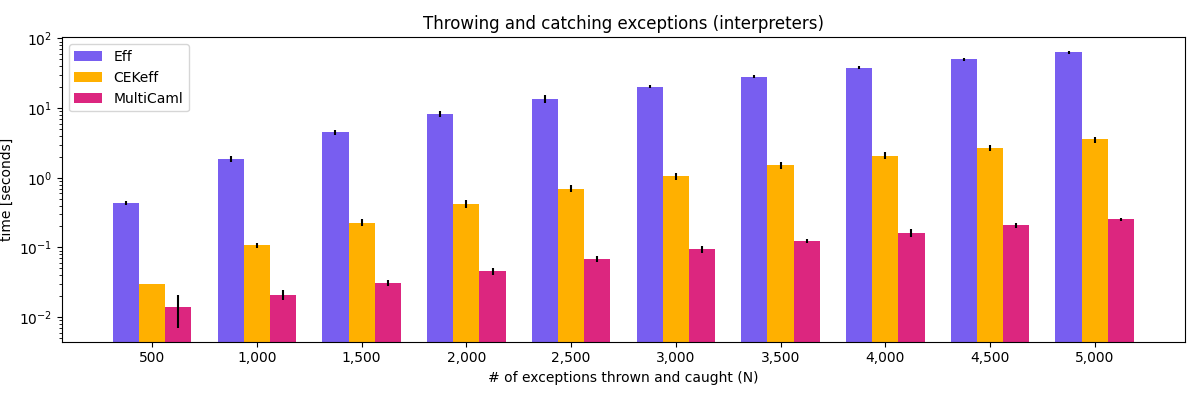
\includegraphics[width=40em]{eval_plots/interp_exception.png}
    \caption{The CEK interpreter performs better than Eff but worse than Multicore OCaml}
    \label{fig:exception-interpreters}
\end{figure}

Athough the OCaml interpreter beats the CEK interpreter in this benchmark, the performance of the SHADE VM
is comparable to MultiCaml's VM even though the execution time for SHADE includes the compilation time to SHADEcode,
but the times for MultiCaml do not include compilation. The reason why this is so is simple: I did not implement
serialization for my byte code and the compilation time is less and less significant as we increase the number of exceptions.

\begin{figure}
    \centering
    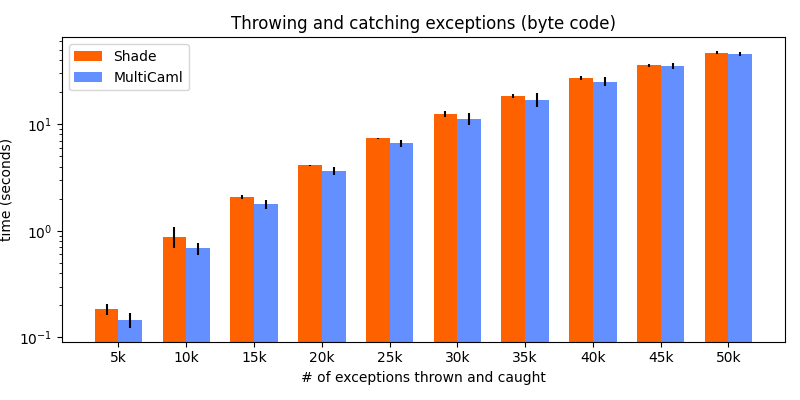
\includegraphics[width=35em]{eval_plots/comp_exception.png}
    \caption{The peformance of SHADE is comparable to Multicore OCaml's}
    \label{fig:exception-bytecode}
\end{figure}

Note that as the byte code solutions are vastly more efficient than their interpreter counterparts they are compared with a larger number of exceptions.
It takes around 63 seconds for the Eff interpreter to evaluate the benchmark with 5000 exceptions, whereas this takes only
3.5 seconds for the CEK interpreter. For SHADE VM the same takes around 200 miliseconds (with compilation included),
which is a 300-fold improvement!

\section{State and I/O}

The state benchmark implements
an integer state and increments it every time the \verb|Incr| effect is performed. The handler of the \verb|Incr| effect
resumes the continuation exactly once. The reason why I chose such a simple computationally cheap operation as integer addition
was that I wanted to measure the performance of performing effects and resuming continuations. As $N$ increases we can be confident
that the cost of performing effects and resuming continuations will dominate the execution time.

\begin{figure}
    \centering
    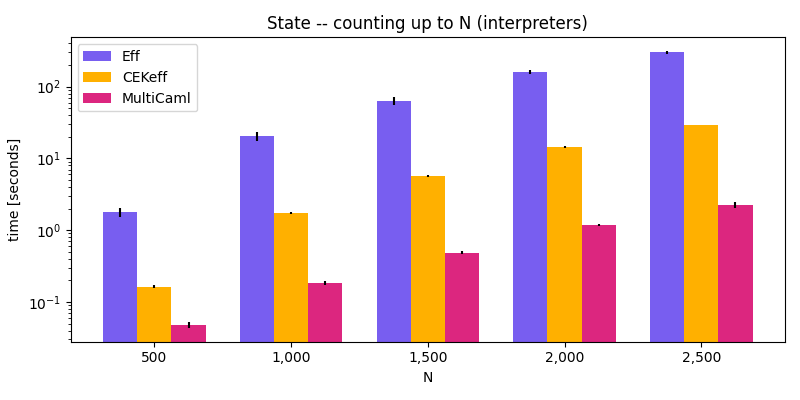
\includegraphics[width=35em]{eval_plots/interp_state.png}
    \caption{Again, the CEK interpreter performs better than Eff but worse than the interpreter of Multicore OCaml}
    \label{fig:state-interpreters}
\end{figure}

\begin{figure}
    \centering
    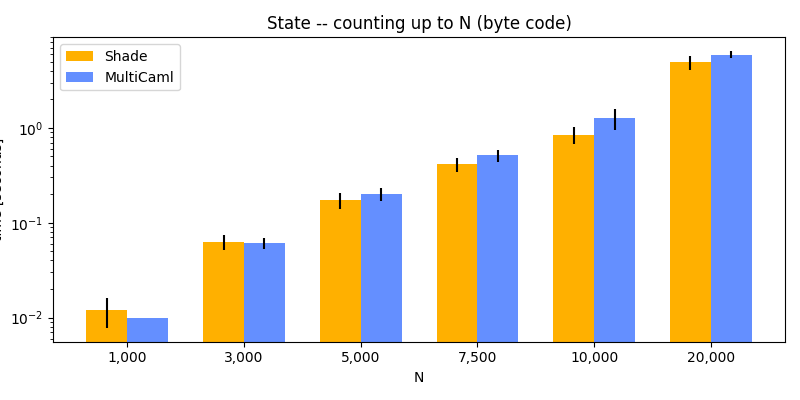
\includegraphics[width=35em]{eval_plots/comp_state.png}
    \caption{SHADE VM's performance is still head-to-head with Multicore OCaml}
    \label{fig:state-bytecode}
\end{figure}

\section{Non-determinism -- Solving the N-queens problem}

The $N$-queens
\footnote{The N-queens problem is concerned with finding the positions of $N$ queens on an $N \times N$ chessboard
such that no two queens attack each other.}
benchmark is a backtracking program which can resume continuations up to $N$ times. Here I don't compare against the CEK interpreter
for the bigger benchmarks because due to its naïve implementation it slows down significantly after $N > 14$. However, the performance of
SHADE VM remains acceptable, but significantly worse than the VM of Multicore OCaml.

\begin{figure}
    \centering
    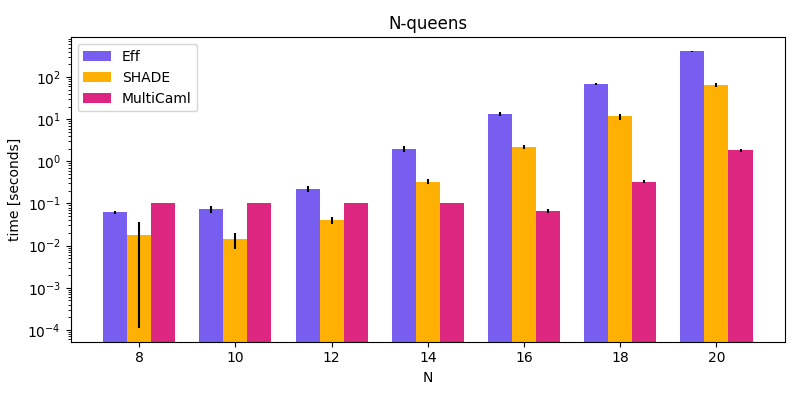
\includegraphics[width=35em]{eval_plots/comp_queens.png}
    \caption{SHADE VM loses against Multicore OCaml here but is still more performant than the Eff interpreter}
    \label{fig:n-queens}
\end{figure}

The reason why Multicore OCaml performs so much better than SHADE VM is what I already mentioned in the Implementation chapter. Multicore OCaml
implements one-shot continuations and relies on the user to specify when a continuation should be cloned.

\mylisting{caml}
{Cloning continuations must be done explicitly in Multicore OCaml}
{lst:multicaml-cloning}
{../code_examples/multicaml_cloning.ml}

\section{Concurrency -- Hello Online World!}

\begin{figure}
    \centering
    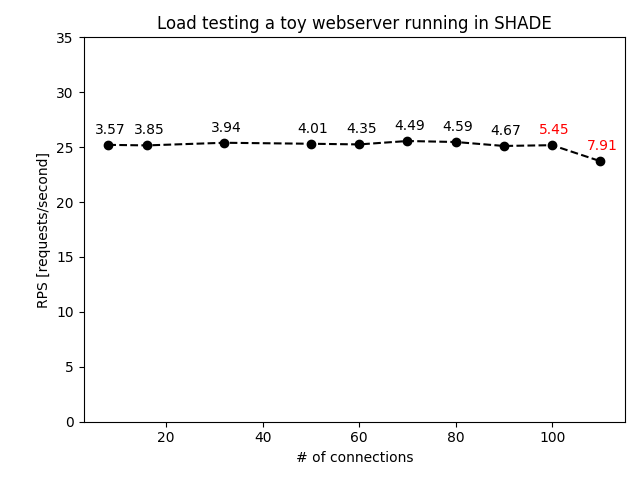
\includegraphics[width=35em]{eval_plots/webserver.png}
    \caption{Although the performance of the webserver is not wonderful, it is my own runtime system that implements it and it can still handle ~100 connections with a p90 time of 5 seconds with a throughput of 25 requests per second.}
    \label{fig:hello-online-world}
\end{figure}

\section{Summary}

\end{document}